\chapter{Исследовательский раздел}

\section{Доступные команды и параметры}

%Интерфейс для управления межсетевым экраном, реализованном в виде загружаемого модуля ядра, представляется файлом firewall\_interface.exe. Чтобы посмотреть доступные команды, необходимо вызвать его без команд или с командой \textbf{help}.  Результат представлен на рисунке \ref{img:commands}

Для просмотра всех доступных команд и параметров следует вызвать команду \textbf{help}.


\begin{figure}[h!]
	\begin{center}
		{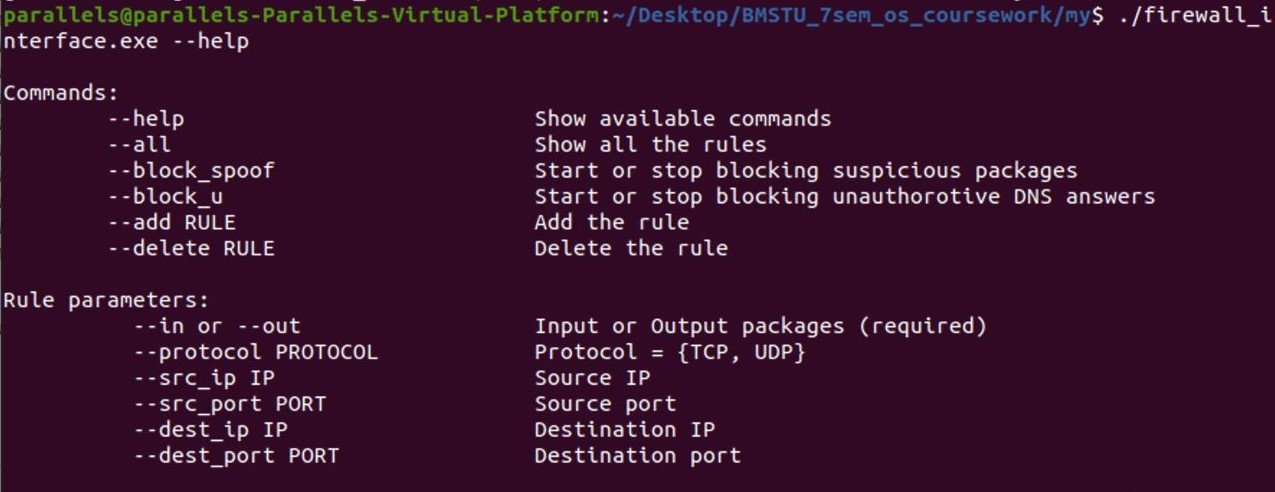
\includegraphics[scale = 0.5]{inc/img/commands.png}}
		\caption{Вывод команды help}
		\label{img:commands}
	\end{center}
\end{figure}


Команды \textbf{help}, \textbf{all}, \textbf{block\_spoof} и \textbf{block\_u} вызываются без параметров, а для команд \textbf{add} и \textbf{delete} необходимо указать параметры добавляемого или удаляемого правила: обязательный параметр -- направление (in или out), а также произвольное количество  необязательных параметров:
\begin{itemize}
	\item протокол (TCP или UDP);
	\item ip-адрес источника;
	\item порт источника;
	\item ip-адрес назначения;
	\item порт назначения.
\end{itemize}

\section{Тестирование фильтрации по ip-адресу}

После загрузки модуля список правил пуст, в чем можно убедиться вызовом команды~\textbf{all}~(рисунок~\ref{img:ip_fw_before}). 
	
\begin{figure}[h!]
	\begin{center}
		{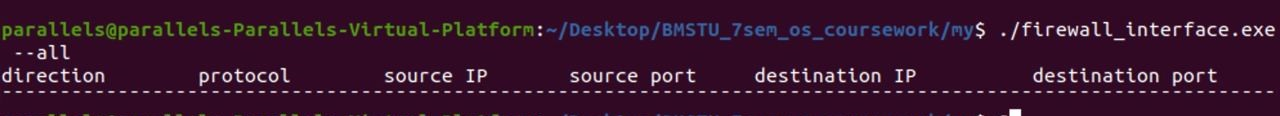
\includegraphics[scale = 0.35]{inc/img/ip_fw_before.jpg}}
		\caption{Вывод команды all}
		\label{img:ip_fw_before}
	\end{center}
\end{figure}

При пустом списке правил была вызвана утилита \textbf{ping} для проверки соединения с устройством с ip-адресом 127.0.0.8. Результат вызова приведен на рисунке~\ref{img:ip_ping_before}: пакеты были успешно отправлены.

\begin{figure}[h!]
	\begin{center}
		{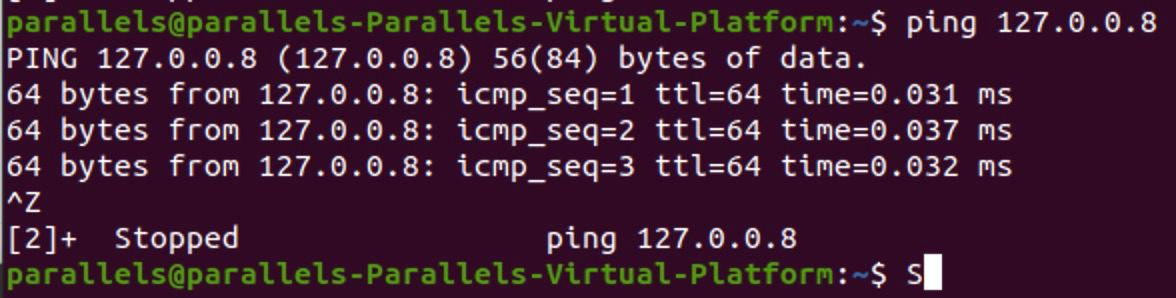
\includegraphics[scale = 0.4]{inc/img/ip_ping_before.jpg}}
		\caption{Вывод утилиты ping до добавления правила}
		\label{img:ip_ping_before}
	\end{center}
\end{figure}

Было добавлено правило фильтрации входящих пакетов по ip-адресу назначения~(рисунок~\ref{img:ip_rule}).

\begin{figure}[h!]
	\begin{center}
		{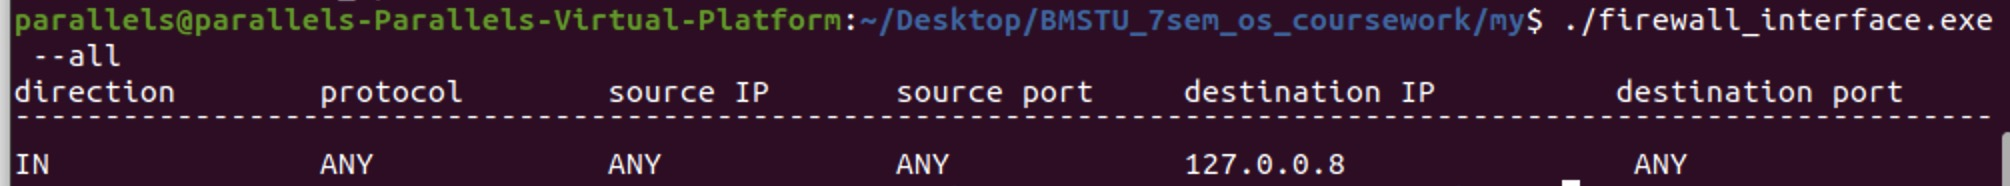
\includegraphics[scale = 0.2]{inc/img/ip_rule.jpg}}
		\caption{Добавленное правило фильтрации}
		\label{img:ip_rule}
	\end{center}
\end{figure}


\clearpage
При вызове \textbf{ping} для проверки соединения с тем же устройством после добавления правила пакеты не были доставлены (рисунок~\ref{img:ip_ping_middle}).

\begin{figure}[h!]
	\begin{center}
		{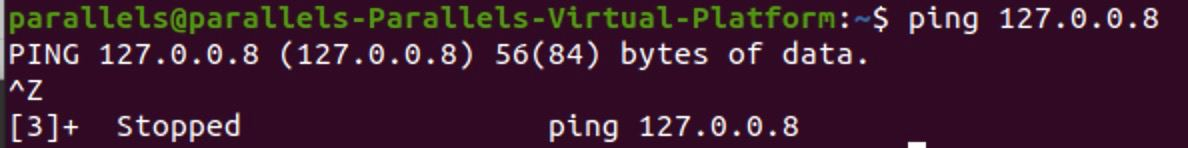
\includegraphics[scale = 0.35]{inc/img/ip_ping_middle.jpg}}
		\caption{Вывод утилиты ping после добавления правила}
		\label{img:ip_ping_middle}
	\end{center}
\end{figure}

Сообщения межсетевого экрана об отброшенных пакетах приведены на рисунке~\ref{img:ip_mes}.

\begin{figure}[h!]
	\begin{center}
		{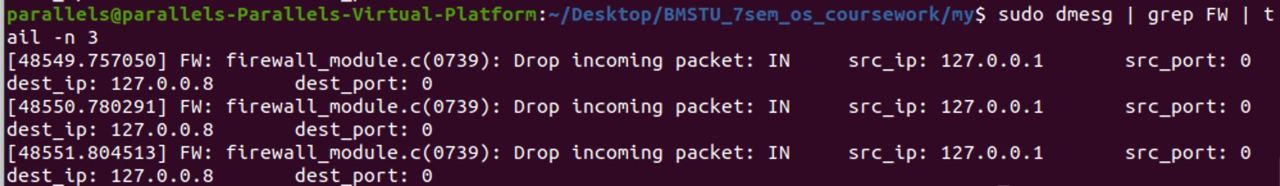
\includegraphics[scale = 0.35]{inc/img/ip_mes.jpg}}
		\caption{Сообщения межсетевого экрана об отброшенных пакетах}
		\label{img:ip_mes}
	\end{center}
\end{figure}

После удаления правила (рисунок~\ref{img:ip_delete}) пакеты вновь успешно доставляются по указанному адресу (рисунок~\ref{img:ip_ping_after}).


\begin{figure}[h!]
	\begin{center}
		{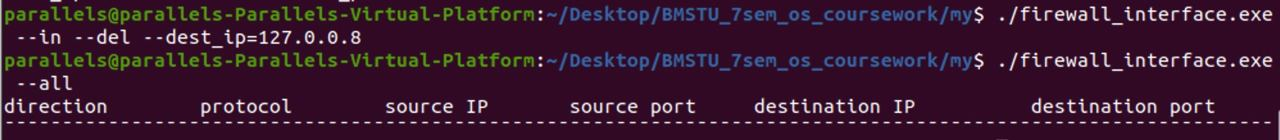
\includegraphics[scale = 0.35]{inc/img/ip_delete.jpg}}
		\caption{Удаление правила}
		\label{img:ip_delete}
	\end{center}
\end{figure}


\begin{figure}[h!]
	\begin{center}
		{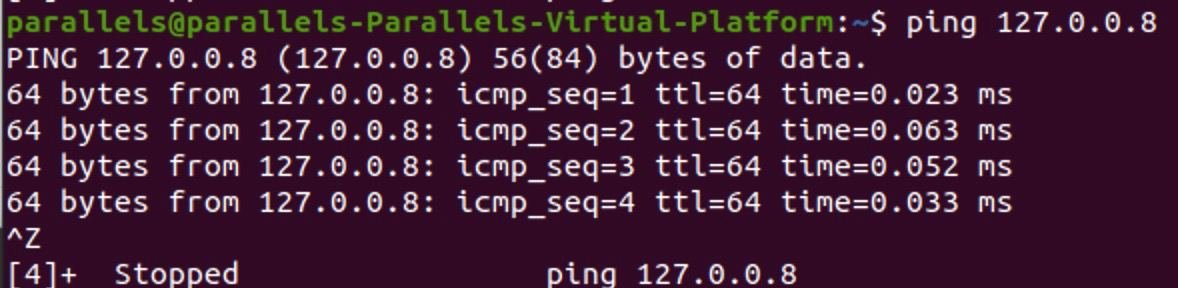
\includegraphics[scale = 0.35]{inc/img/ip_ping_after.jpg}}
		\caption{Вывод утилиты ping после удаления правила}
		\label{img:ip_ping_after}
	\end{center}
\end{figure}


\section{Тестирование фильтрации по протоколу}

Для тестирования фильтрации по протоколу была использована программа \textbf{Wireshark}. До добавления правила фильтрации регулярно происходил обмен пакетами по протоколу TCP~(рисунок~\ref{img:tcp_before}). 

\begin{figure}[h!]
	\begin{center}
		{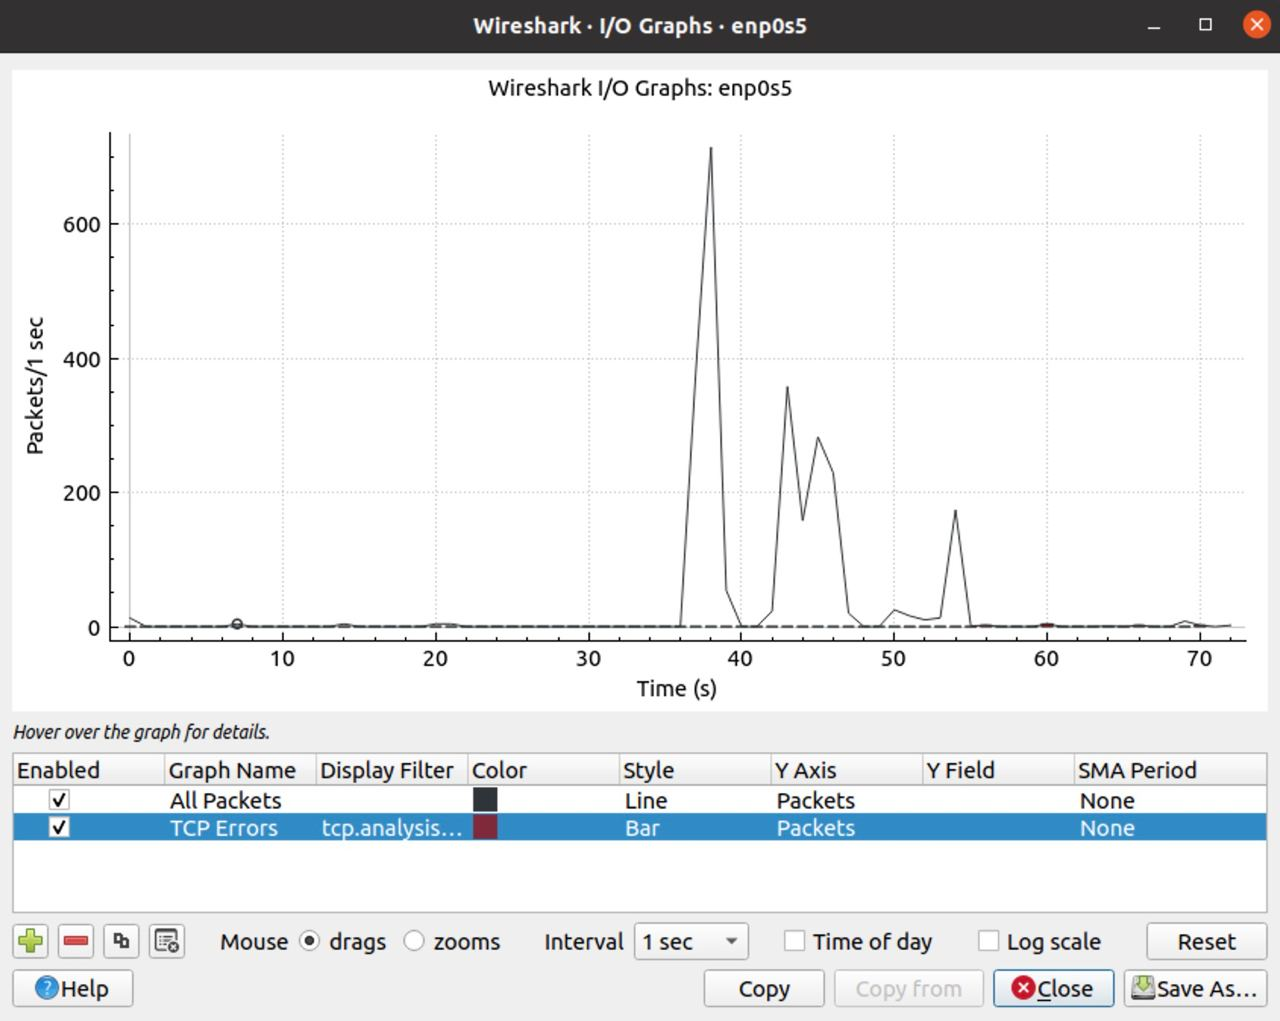
\includegraphics[scale = 0.3]{inc/img/tcp_before.jpg}}
		\caption{Обмен пакетами по протоколу TCP до добавления правила}
		\label{img:tcp_before}
	\end{center}
\end{figure}

После добавления правил фильтрации, согласно которым необходимо отбрасывать все передаваемые по протоколу TCP пакеты~(рисунок~\ref{img:tcp_rule}), обмен такими пакетами практически прекратился, что продемонстрировано на рисунке~\ref{img:tcp_middle}.


\begin{figure}[h!]
	\begin{center}
		{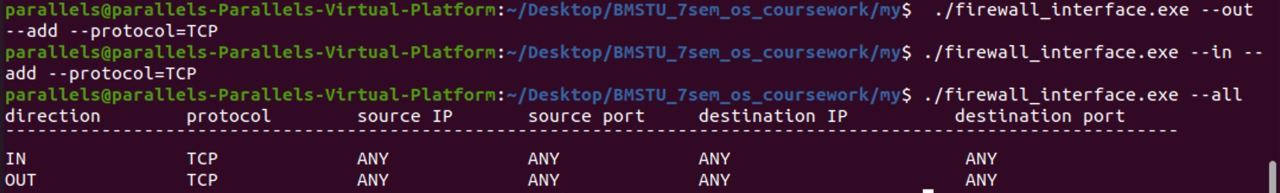
\includegraphics[scale = 0.35]{inc/img/tcp_rule.jpg}}
		\caption{Добавление правил фильтрации по протоколу TCP}
		\label{img:tcp_rule}
	\end{center}
\end{figure}

\clearpage
\begin{figure}[h!]
	\begin{center}
		{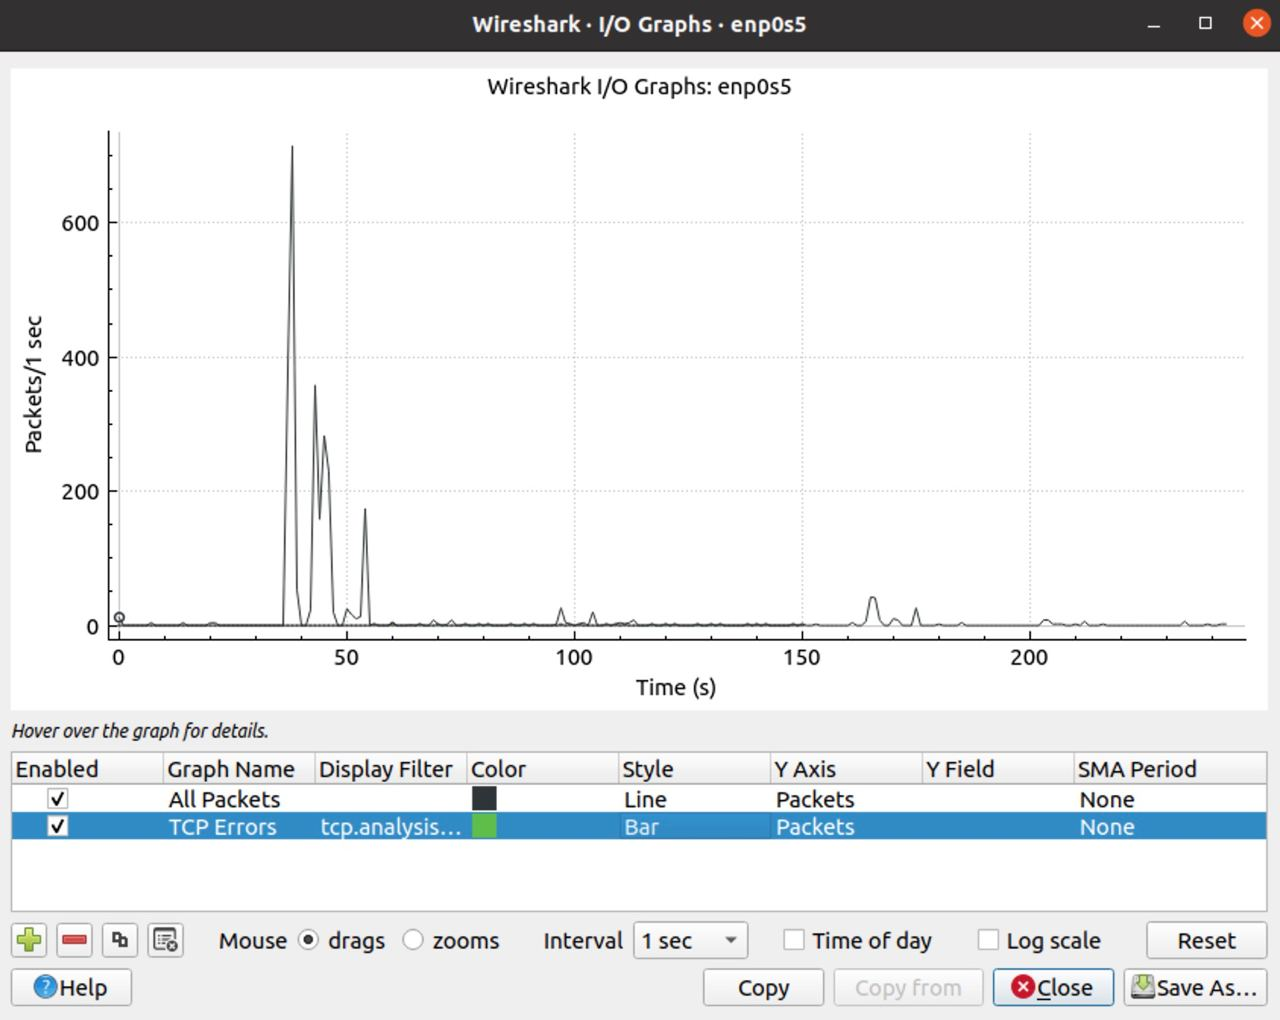
\includegraphics[scale = 0.3]{inc/img/tcp_middle.jpg}}
		\caption{Обмен пакетами по протоколу TCP после добавления правил}
		\label{img:tcp_middle}
	\end{center}
\end{figure}

Соответствующие сообщения об отброшенных пакетах от межсетевого экрана приведены на рисунке~\ref{img:tcp_mess}.


\begin{figure}[h!]
	\begin{center}
		{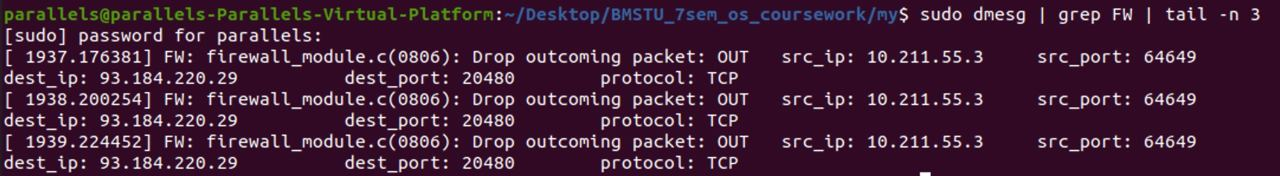
\includegraphics[scale = 0.35]{inc/img/tcp_mess.jpg}}
		\caption{Сообщения об отброшенных пакетах от межсетевого экрана}
		\label{img:tcp_mess}
	\end{center}
\end{figure}

\clearpage
После удаления правил~(рисунок~\ref{img:tcp_delete}) обмен пакетами возобновился~(рисунок \ref{img:tcp_after}).


\begin{figure}[h!]
	\begin{center}
		{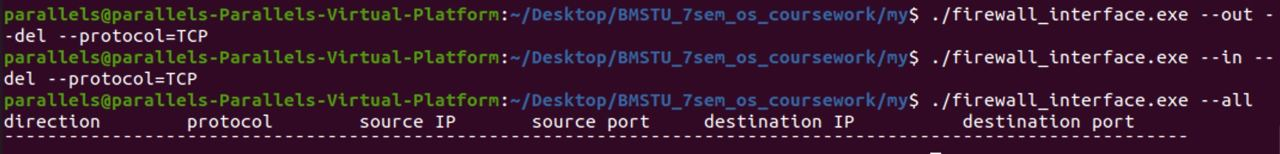
\includegraphics[scale = 0.35]{inc/img/tcp_delete.jpg}}
		\caption{Удаление правил фильтрации по протоколу TCP}
		\label{img:tcp_delete}
	\end{center}
\end{figure}


\begin{figure}[h!]
	\begin{center}
		{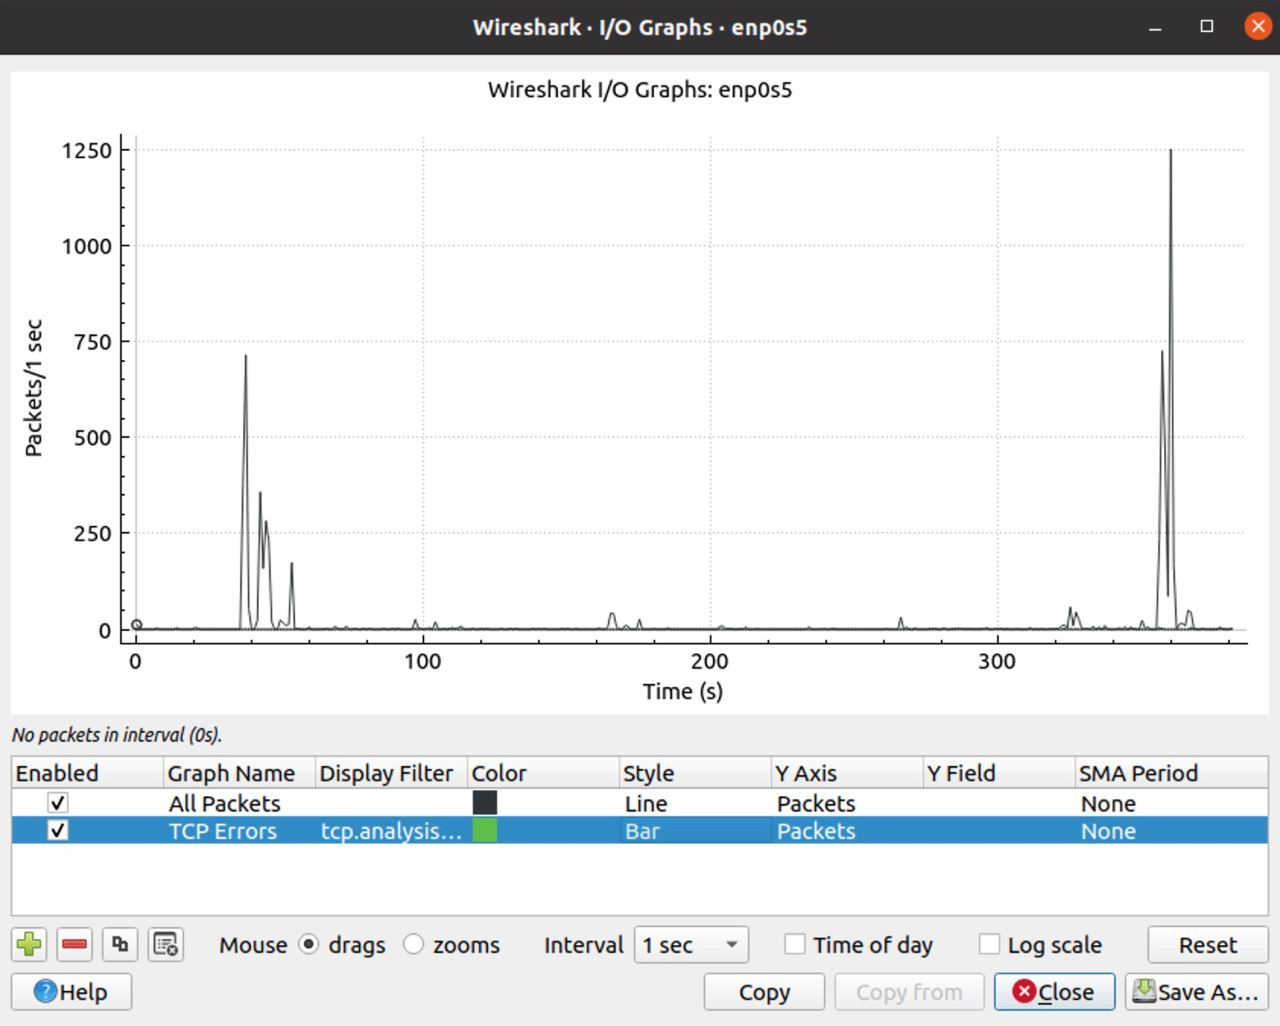
\includegraphics[scale = 0.3]{inc/img/tcp_after.jpg}}
		\caption{Обмен пакетами по протоколу TCP после удаления правил}
		\label{img:tcp_after}
	\end{center}
\end{figure}



\section{Вывод информации о DNS-пакетах}

Для тестирования вывода информации о DNS-пакетах было произведено обращение по доменному имени bmstu.ru~(рисунок~\ref{img:dns_bmstu}). 

\clearpage
\begin{figure}[h!]
	\begin{center}
		{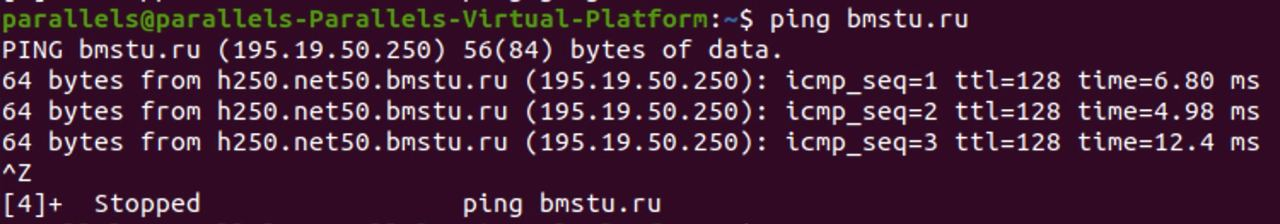
\includegraphics[scale = 0.3]{inc/img/dns_bmstu.jpg}}
		\caption{Обращение по доменному имени bmstu.ru}
		\label{img:dns_bmstu}
	\end{center}
\end{figure}


На рисунках~\ref{img:dns_query}~и~\ref{img:dns_response} приведен частичный вывод информации о пакете-запросе и пакете-ответе, соответственно.


\begin{figure}[h!]
	\begin{center}
		{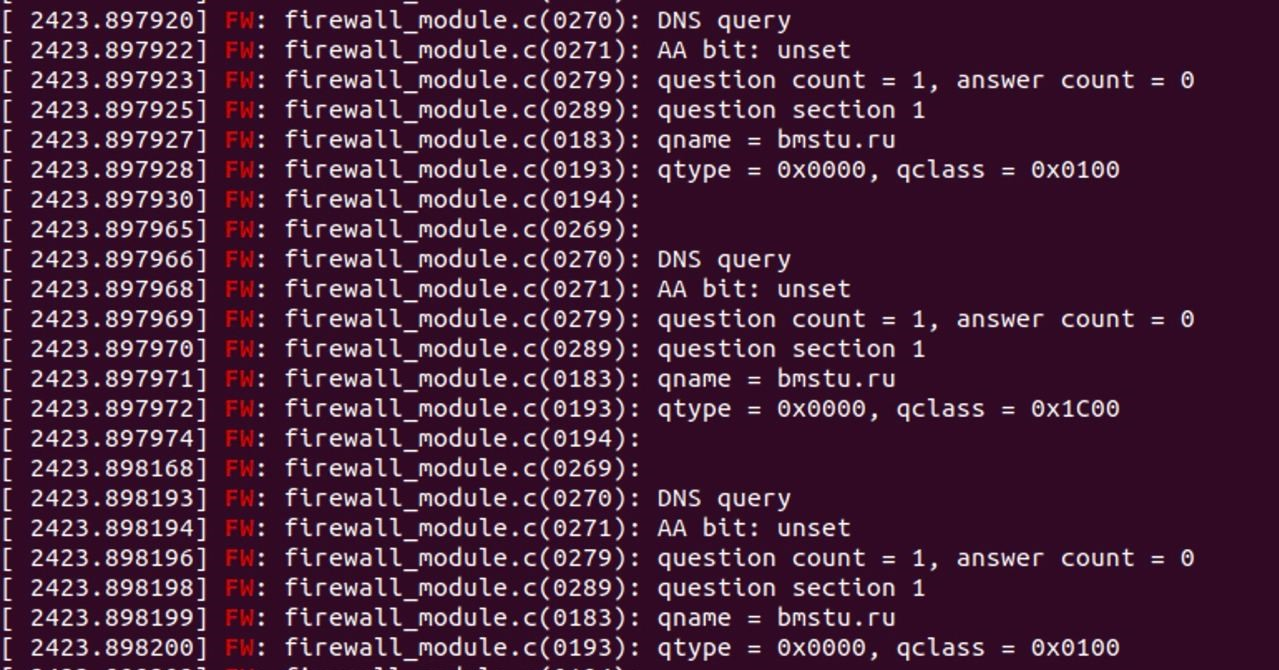
\includegraphics[scale = 0.4]{inc/img/dns_query.jpg}}
		\caption{Информации о пакете-запросе}
		\label{img:dns_query}
	\end{center}
\end{figure}


\begin{figure}[h!]
	\begin{center}
		{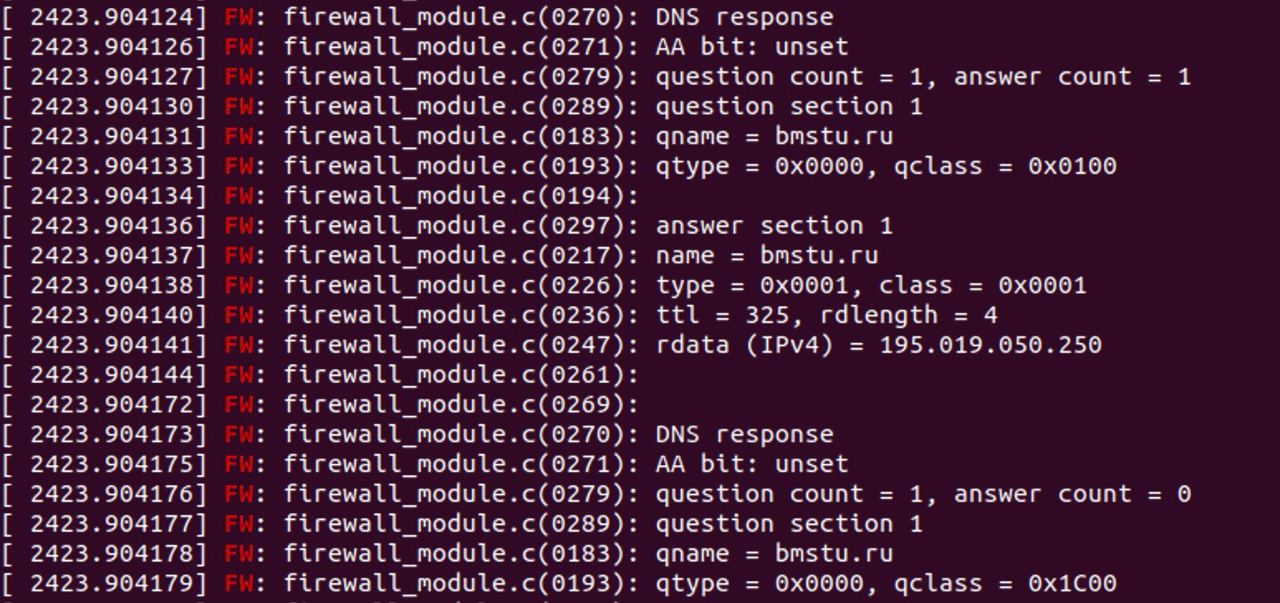
\includegraphics[scale = 0.3]{inc/img/dns_response.jpg}}
		\caption{Информации о пакете-ответе}
		\label{img:dns_response}
	\end{center}
\end{figure}


\section{Тестирование запрета приема ответов от неавторитетных DNS-серверов}

До включения запрета приема ответов от неавторитетных DNS-серверов было произведено обращение по доменному имени google.com, и соединение было успешно установлено~(рисунок~\ref{img:u_before}). 

\begin{figure}[h!]
	\begin{center}
		{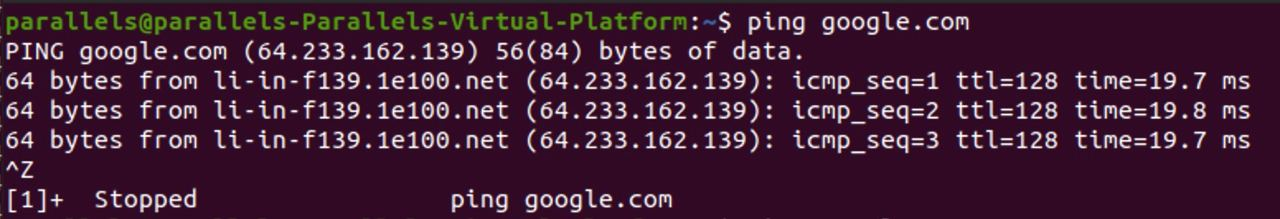
\includegraphics[scale = 0.35]{inc/img/u_before.jpg}}
		\caption{Обращение по доменному имени google.com до включения запрета}
		\label{img:u_before}
	\end{center}
\end{figure}


Затем был включен запрет приема ответов от неавторитетных DNS-серверов~(рисунок~\ref{img:u_on}). 

\begin{figure}[h!]
	\begin{center}
		{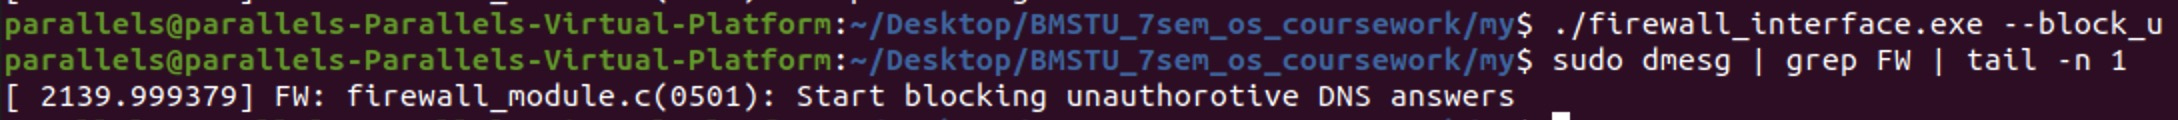
\includegraphics[scale = 0.2]{inc/img/u_on.jpg}}
		\caption{Включение запрета приема ответов от неавторитетных DNS-серверов}
		\label{img:u_on}
	\end{center}
\end{figure}

После включения запрета при обращении по тому же доменному имени был получен ответ от неавторитетного DNS-сервера, в результате чего пакет был отброшен~(рисунок~\ref{img:u_mess}), а соединение не было установлено~(рисунок~\ref{img:u_middle})


\begin{figure}[h!]
	\begin{center}
		{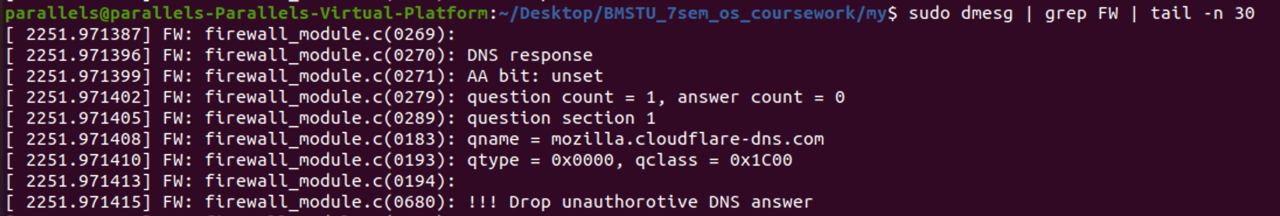
\includegraphics[scale = 0.35]{inc/img/u_mess.jpg}}
		\caption{Сообщение от межсетевого экрана об отброшенном пакете от неавторитетного DNS-сервера}
		\label{img:u_mess}
	\end{center}
\end{figure}

\clearpage
\begin{figure}[h!]
	\begin{center}
		{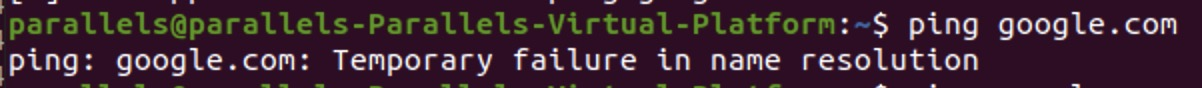
\includegraphics[scale = 0.3]{inc/img/u_middle.jpg}}
		\caption{Обращение по доменному имени google.com после включения запрета}
		\label{img:u_middle}
	\end{center}
\end{figure}

При снятии запрета~(рисунок~\ref{img:u_off}) соединение вновь устанавливается успешно~(рисунок~\ref{img:u_after}).  


\begin{figure}[h!]
	\begin{center}
		{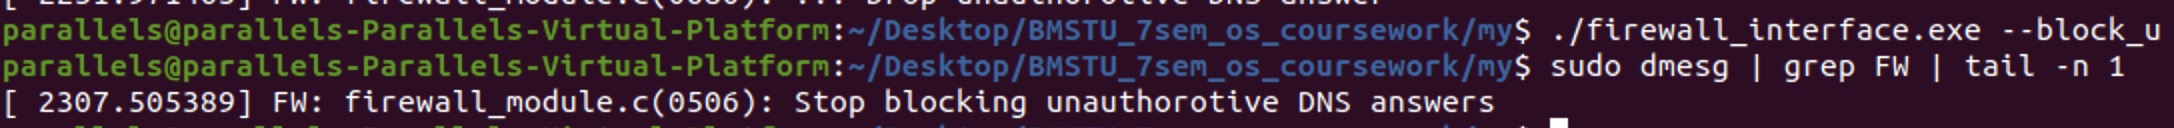
\includegraphics[scale = 0.2]{inc/img/u_off.jpg}}
		\caption{Снятие запрета на прием пакетов от неавторитетных DNS-серверов}
		\label{img:u_off}
	\end{center}
\end{figure}


\begin{figure}[h!]
	\begin{center}
		{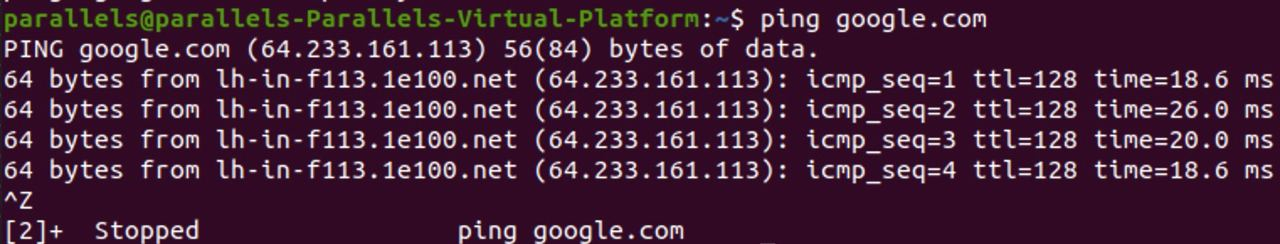
\includegraphics[scale = 0.35]{inc/img/u_after.jpg}}
		\caption{Обращение по доменному имени google.com после снятия запрета}
		\label{img:u_after}
	\end{center}
\end{figure}